\begin{wrapfigure}{r}{0.3\linewidth}
    \centering
    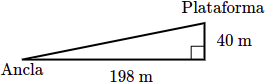
\includegraphics[width=\linewidth]{../images/proverb_pitagoras_03.png}
    \caption{}
    \label{fig:proverb_pitagoras_03}
\end{wrapfigure}
Una tirolesa comienza en una plataforma que está a 40 metros del suelo.
El punto de anclaje de la tirolesa está a 198 metros en dirección horizontal desde la base de la plataforma, como se muestran a continuación en la figura \ref{fig:proverb_pitagoras_03}.
\textbf{¿Qué tan larga es la tirolesa?}
\vspace{2cm}
\begin{solutionbox}{5.5cm}\footnotesize
    Podemos usar el teorema de Pitágoras para obtener $x$.
    La ecuación del teorema de Pitágoras es:
    \[c^2=a^2+b^2\]
    donde $a$ y $b$ son las longitudes de los dos catetos del triángulo y $c$ es la longitud de la hipotenusa.
    En este caso, $a=40$, $b=198$ y $c=x$.
    \begin{align*}
        x^2 & =40^2+198^2     \\
        x^2 & =1,600 + 39,204 \\
        x^2 & =40,804         \\
        x   & =\sqrt{40,804}  \\
        x   & = 202
    \end{align*}
    La longitud de la tirolesa es 202 metros.
\end{solutionbox}